  \section{Protokołu treningowy FL do zadania weryfikacji twarzy}\label{sec:fedfaceid}
  \subsection{Generowanie przykładów negatywnych}
  \subsubsection{StyleGAN}
  \begin{figure}[H]
      \begin{center}
      \renewcommand\tabcolsep{1pt}
      \begin{tabular}{ccc}
        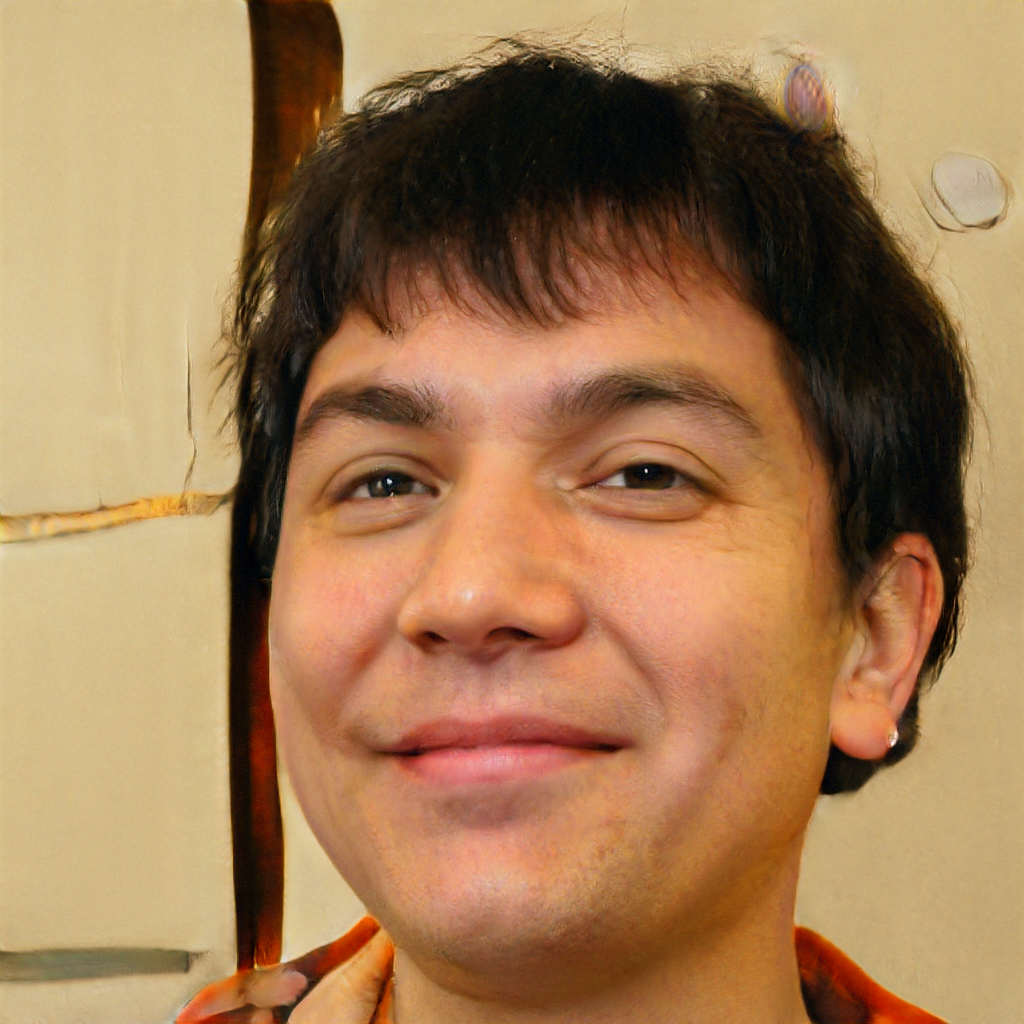
\includegraphics[width=.3\linewidth]{img/gen/1.png} &
        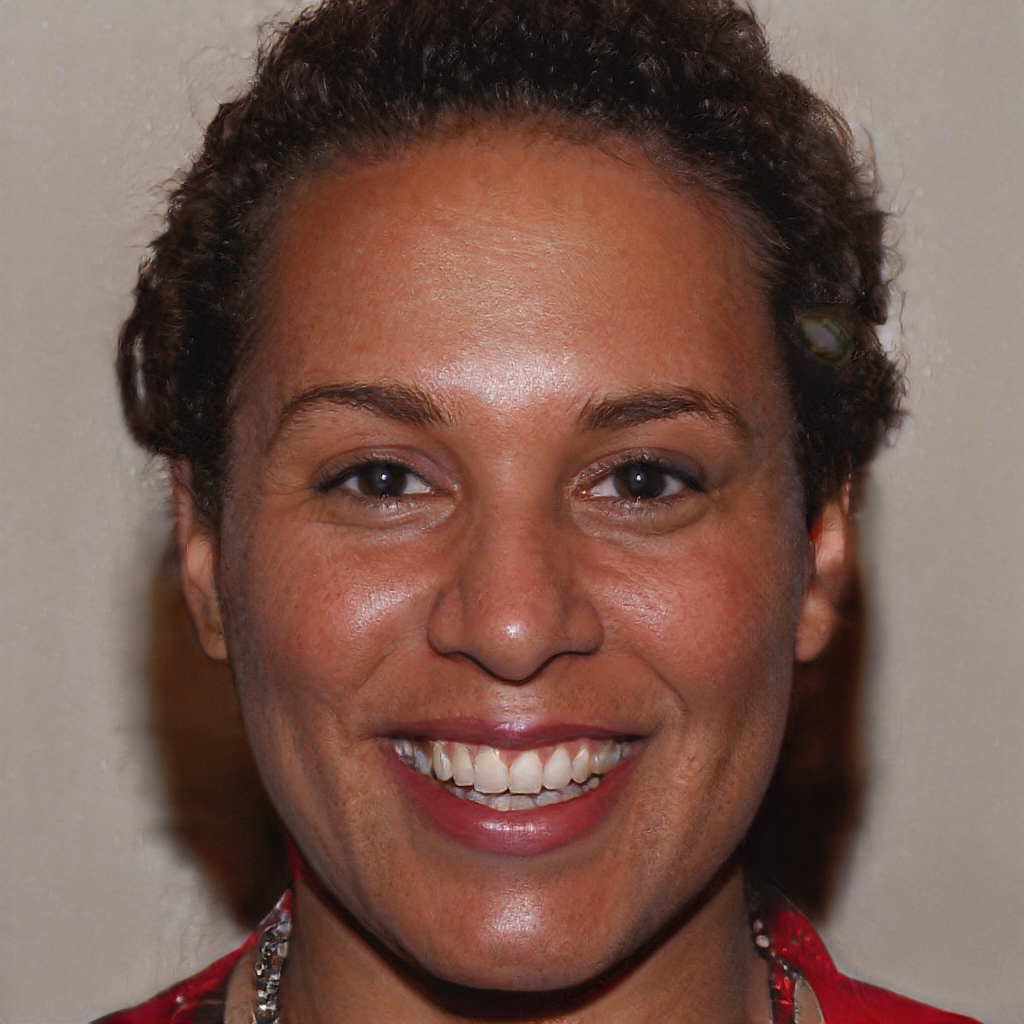
\includegraphics[width=.3\linewidth]{img/gen/2.png} &
        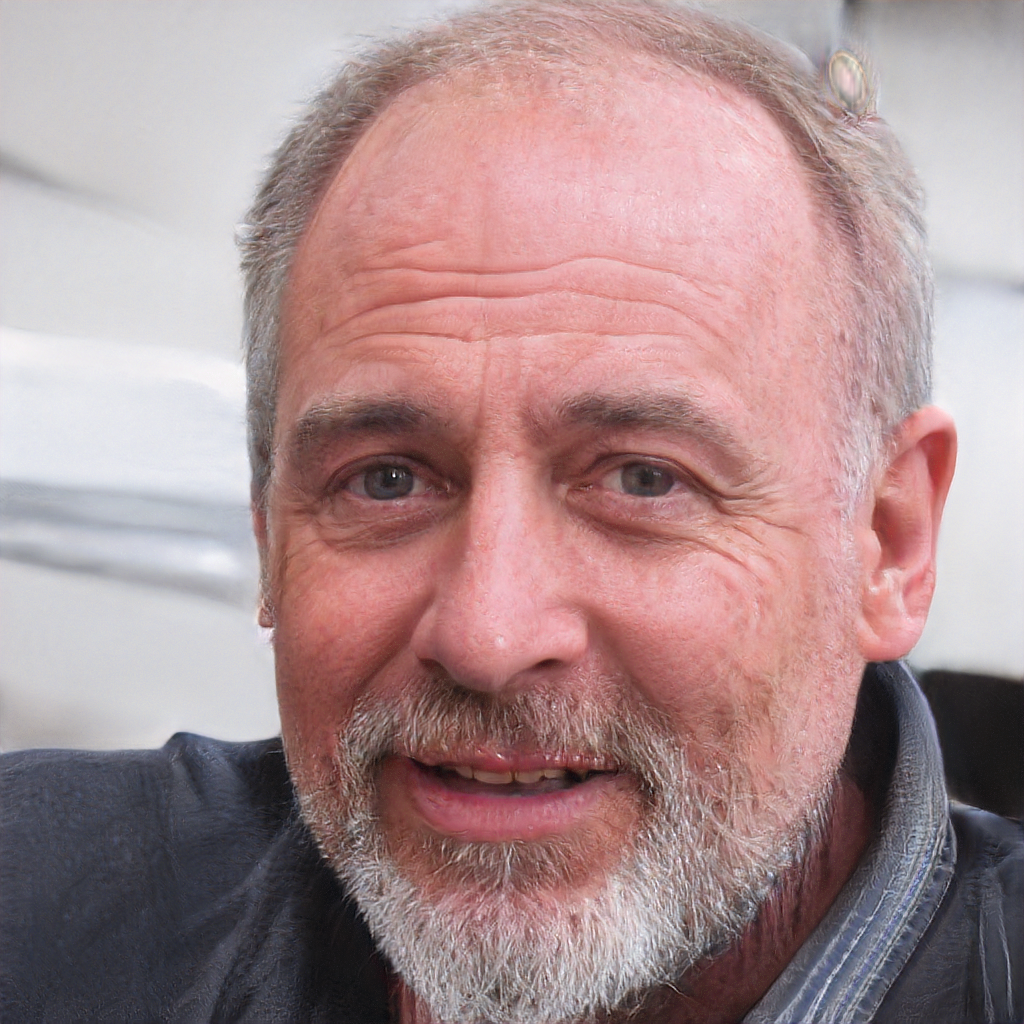
\includegraphics[width=.3\linewidth]{img/gen/3.png} \\
        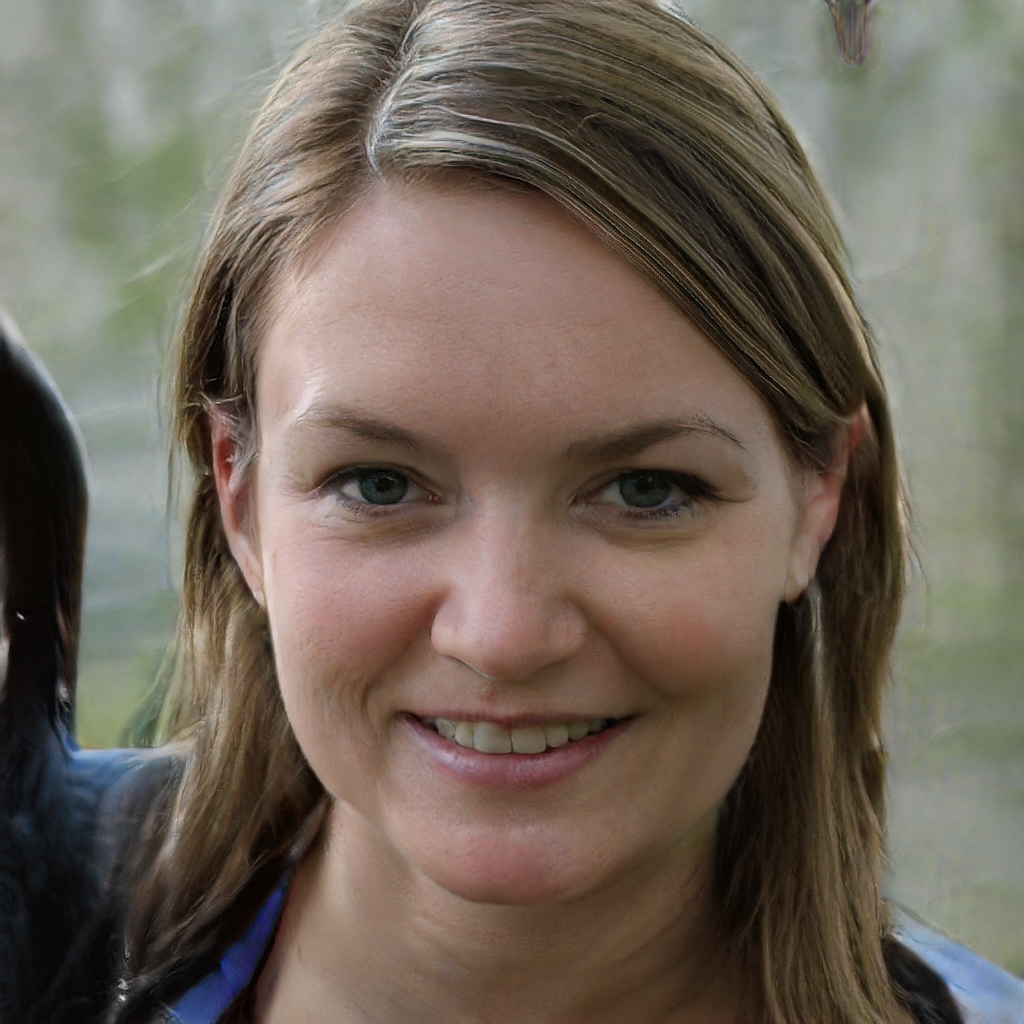
\includegraphics[width=.3\linewidth]{img/gen/4.png} &
        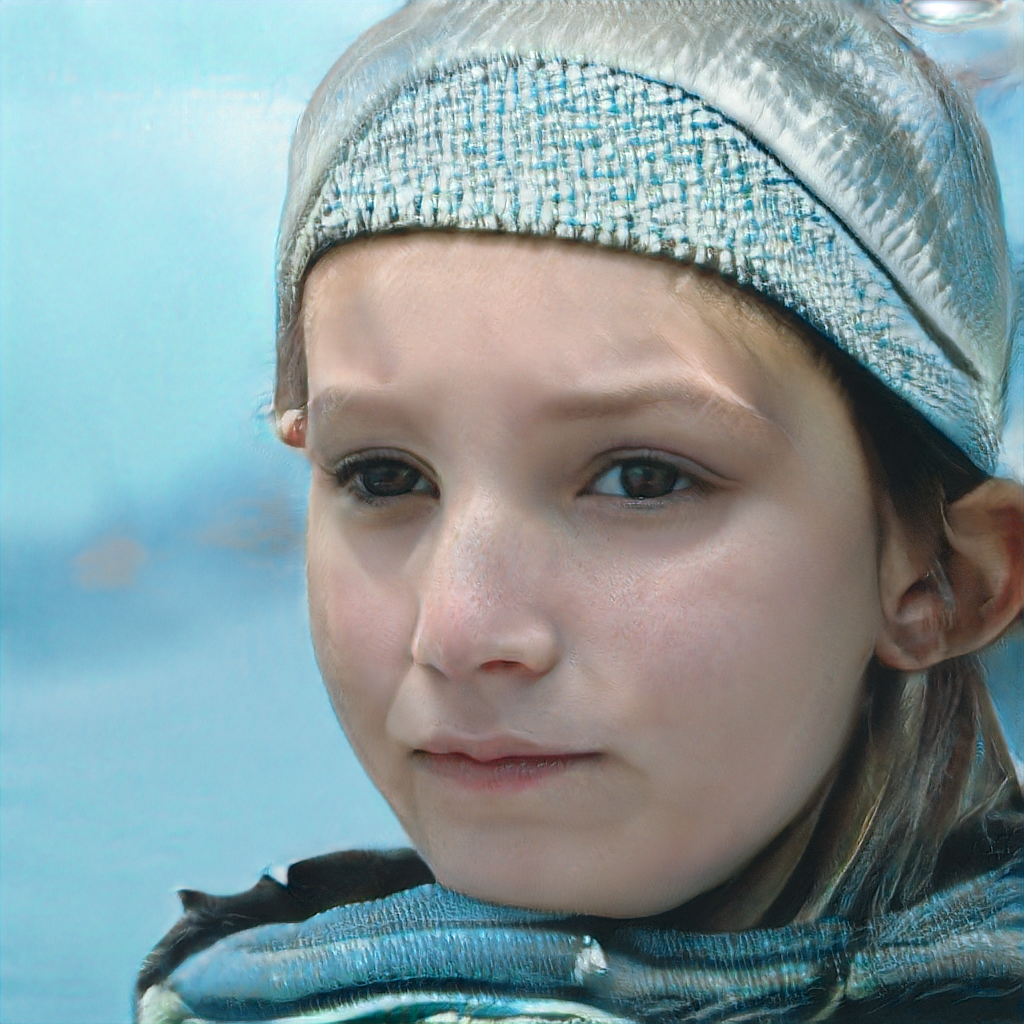
\includegraphics[width=.3\linewidth]{img/gen/5.png} &
        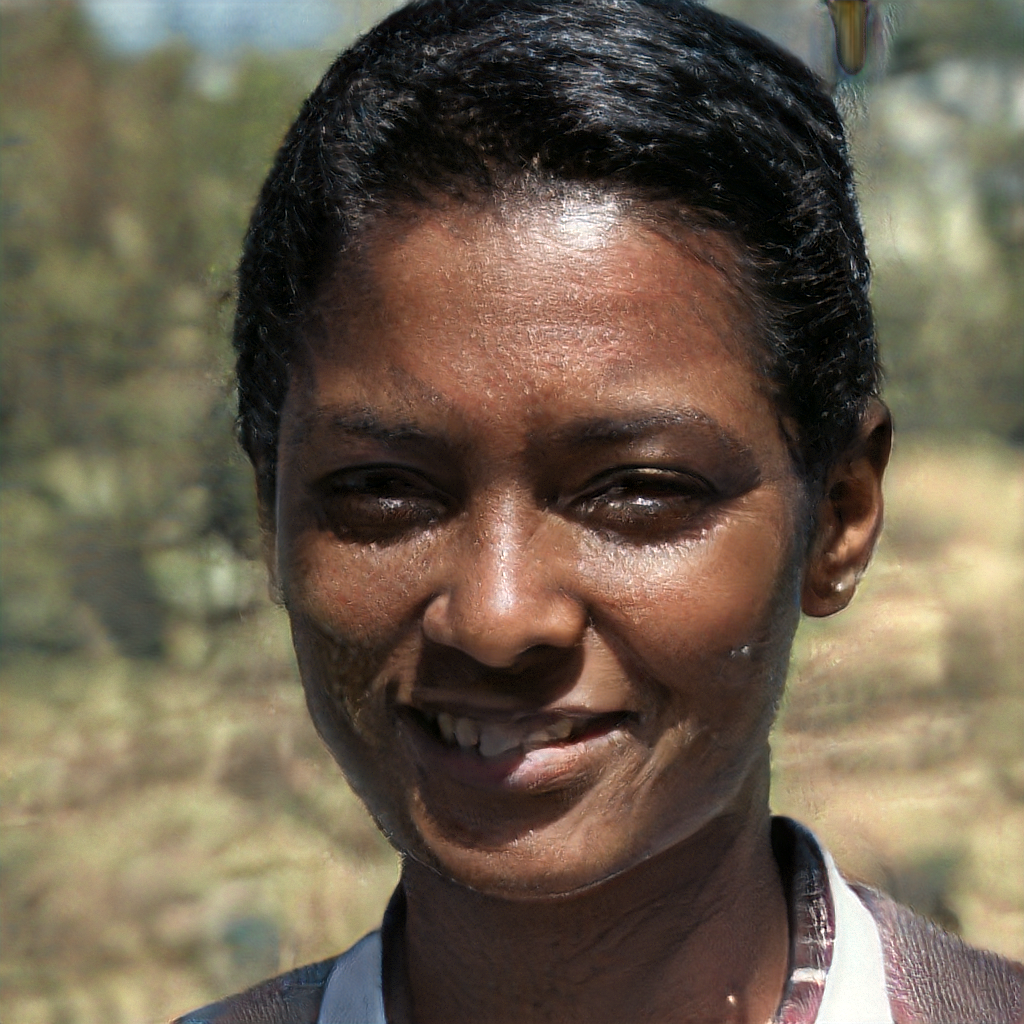
\includegraphics[width=.3\linewidth]{img/gen/6.png} \\
        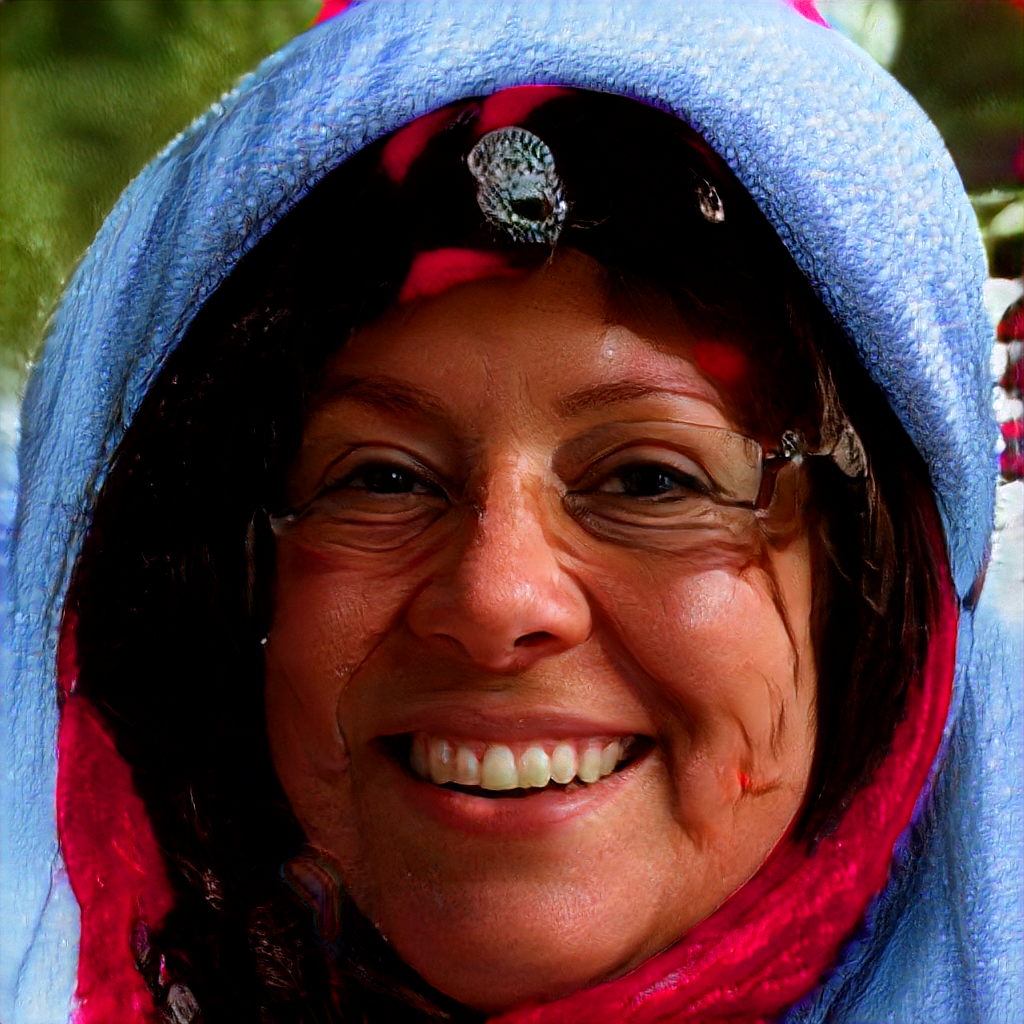
\includegraphics[width=.3\linewidth]{img/gen/7.png} &
        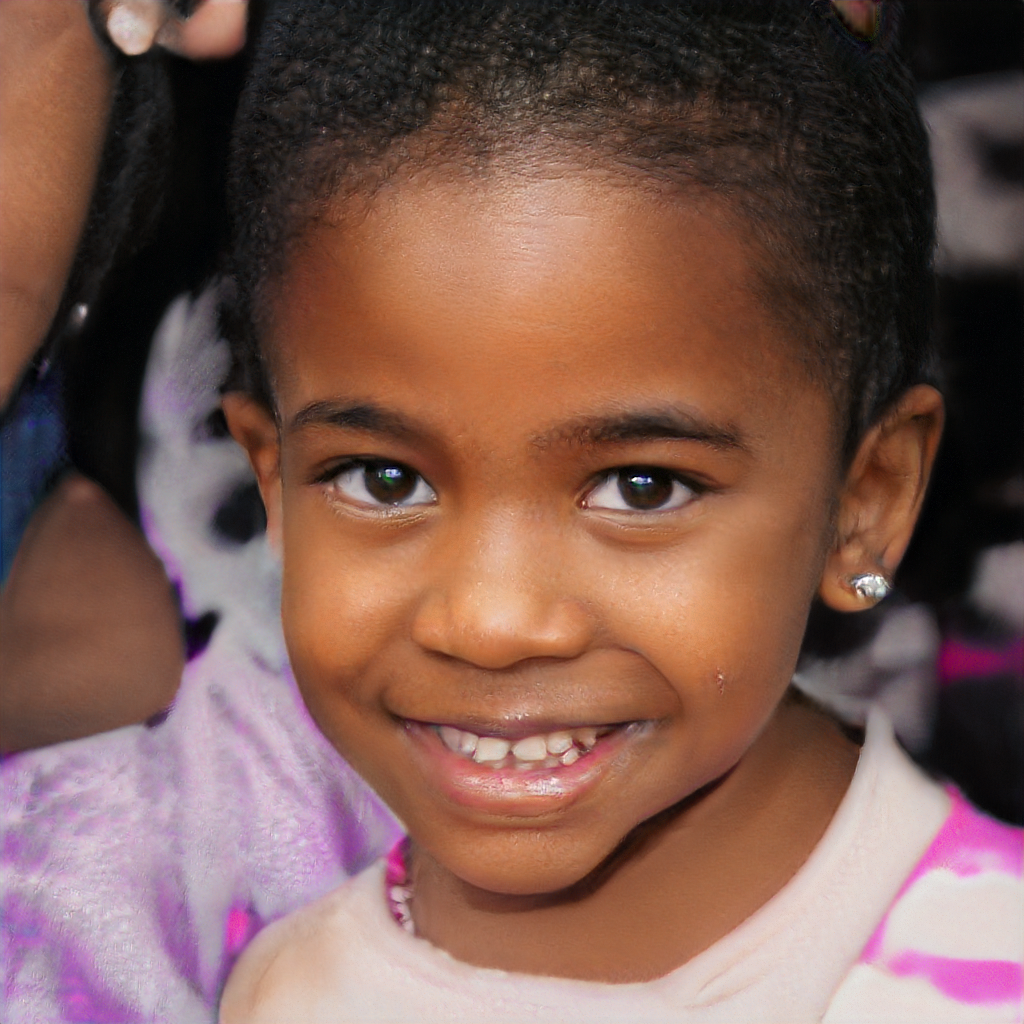
\includegraphics[width=.3\linewidth]{img/gen/8.png} &
        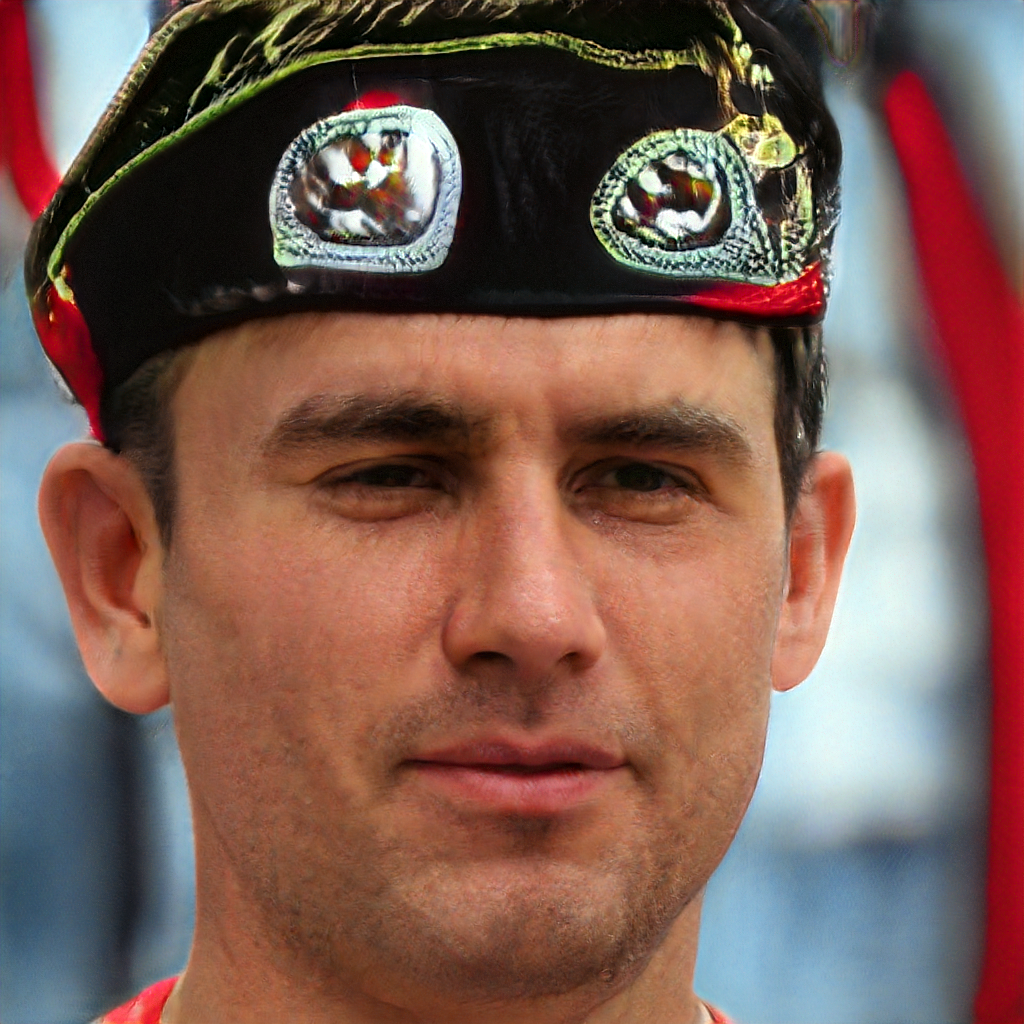
\includegraphics[width=.3\linewidth]{img/gen/9.png} \\
      \end{tabular}
      \end{center}
      \caption{{\bf Przykłady działania generatora twarzy.}}
      \label{fig:generator_twarzy}
    \end{figure}

  \subsection{Zbiory danych}
  \begin{table}[H]
  \begin{center}
  \begin{tabular}{ccccc}
  \hline
  Zbiór danych  & \# osób   &   \# zdjęć  &   \# zdjęć na osobę   &   aligned \\
  \hline
  MS1M-DeepGlint \cite{glintweb}   & 87K  & 3.9M & ?/44.8/? & Tak \\
  \hline
  \hline
  VGGFace2-test-train   & 500 & 163.3K & ?/361/? & Nie  \\
  StyleGAN-0.7   & 1M & 1M & 1 & Nie  \\
  \hline
  \hline
  VGGFace2-test-test    & 500 & 18.1K & ?/361/? & Nie  \\
  \hline
  \end{tabular}
  \end{center}
  \caption{\textbf{Zbiory danych} MS1M-DeepGlint posłuży do wytrenowania ekstraktora cech, a VGGFace2-test po podzieleniu do treningu oraz testowania treningu FL.} \label{table:dataset-FL}
  \vspace{-4mm}
  \end{table}
